\documentclass[11pt]{article}
\usepackage[margin=1in]{geometry}
\usepackage{graphicx}
\usepackage{booktabs}
\usepackage{caption}
\captionsetup{font=small}

\newcommand{\pair}[3]{%
  \begin{figure}[htbp]
  \centering
  {\small Baseline: distributive trade in services, government included\par}
  \vspace{2pt}
  \includegraphics[width=#2\textwidth]{../analysis/results/figures/#1}\par
  \vspace{10pt}
  {\small Experiment: distributive trade in goods, government excluded\par}
  \vspace{2pt}
  \includegraphics[width=#2\textwidth]{../analysis/results/figures_2/#1}
  \caption{#3}
  \end{figure}}

\title{Current Figures}
\author{}
\date{\today}

\begin{document}
\maketitle

\section*{Recovered parameters under the two sector definitions}

Every figure in this section appears twice: the baseline sector definition on
top, and the \texttt{data\_\allowbreak processing\_\allowbreak 2} experiment
below. The two pipelines
read the same raw data and run the same code; they differ only in which sectors
count as goods and whether government consumption is counted.

Input--output tables are recorded at basic prices, so the wholesale and retail
margin on a consumer good is output of the trade sector and lands in services,
while the national accounts count the whole till price as goods. The experiment
moves wholesale and retail trade into goods, together with hotels and
restaurants, which the pre-2000 tables cannot separate from it, and drops
government consumption. That moves about a third of U.S. consumption out of
services and into manufacturing, from 75 percent services in 1965 to 41 percent,
against 48 percent in the BEA data. The recovered parameters follow: the demand
shifters change ordering, so manufacturing starts above services and the two
converge rather than diverging, which is the pattern in the 2017 draft. Trade
costs and productivities move in manufacturing and services and leave
agriculture essentially unchanged, since nothing enters or leaves agriculture.

\begin{table}[htbp]
\centering
\caption{U.S. consumption shares under the two definitions}
\begin{tabular}{lccc ccc}
\toprule
& \multicolumn{3}{c}{Baseline} & \multicolumn{3}{c}{Experiment} \\
\cmidrule(lr){2-4} \cmidrule(lr){5-7}
Year & Agr. & Man. & Serv. & Agr. & Man. & Serv. \\
\midrule
1965 & 0.011 & 0.243 & 0.746 & 0.014 & 0.580 & 0.407 \\
1990 & 0.006 & 0.192 & 0.802 & 0.008 & 0.469 & 0.523 \\
2014 & 0.005 & 0.156 & 0.839 & 0.007 & 0.400 & 0.594 \\
\bottomrule
\end{tabular}
\end{table}

\clearpage
\pair{demand_shifters.pdf}{0.62}{Sectoral demand shifters.}

\clearpage
\pair{trade_costs.pdf}{0.88}{Sectoral trade costs, indexed to 1965.}

\clearpage
\pair{productivities.pdf}{0.50}{Sectoral productivities, 1965 normalized to zero.}

\clearpage
\pair{financial_friction.pdf}{0.80}{Financial friction and net foreign assets.}

\clearpage
\pair{investment_efficiency.pdf}{0.55}{Investment-specific efficiency shifters.}

\clearpage
\pair{investment_shares.pdf}{0.80}{Sectoral investment shares.}

\clearpage
\section*{Counterfactual}

Solved on the baseline data.

\begin{figure}[htbp]
\centering
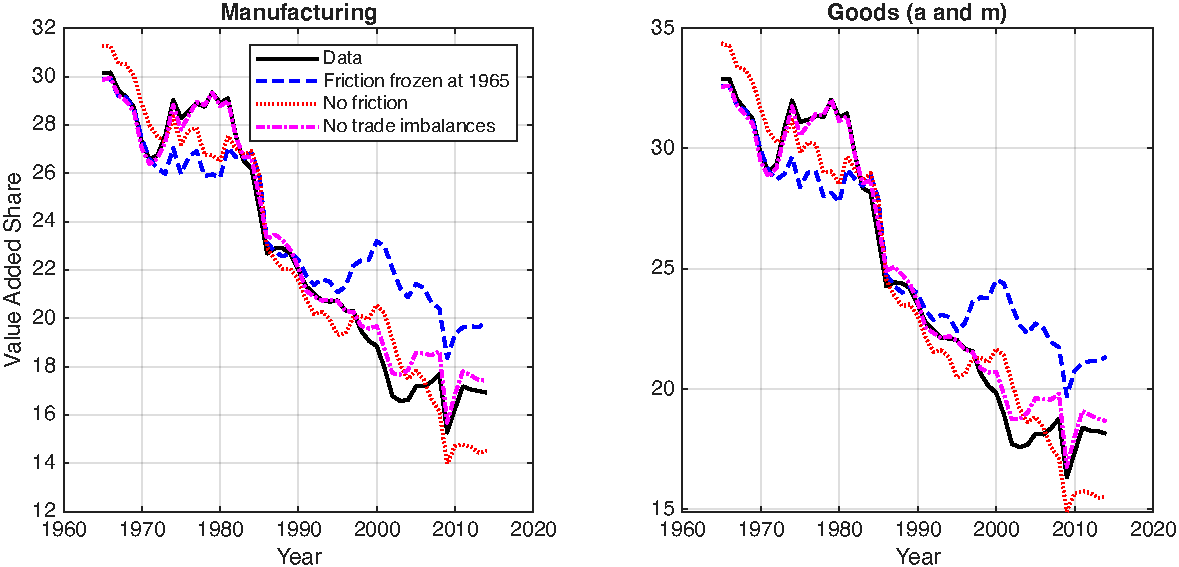
\includegraphics[width=\textwidth]{../analysis/code/model/results/value_added_shares.pdf}
\end{figure}

\begin{figure}[htbp]
\centering
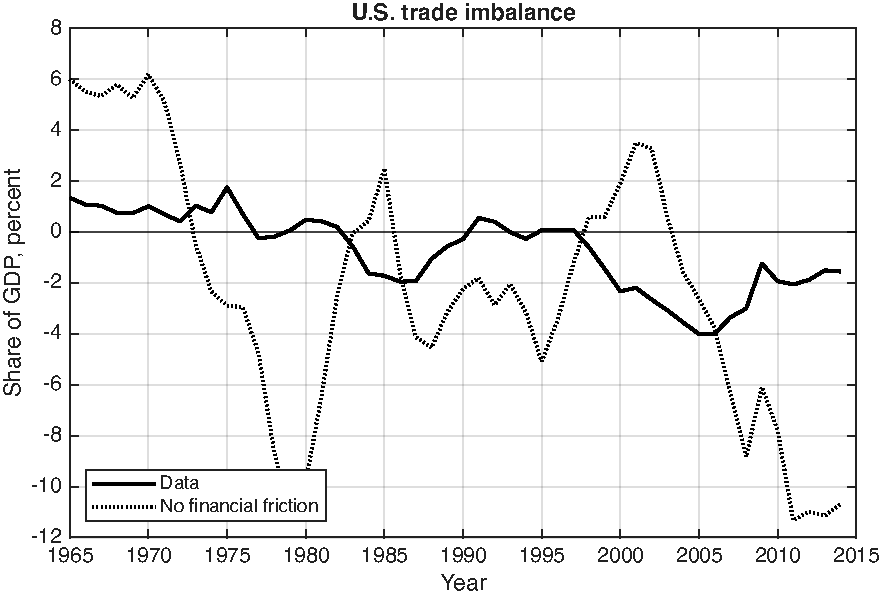
\includegraphics[width=0.75\textwidth]{../analysis/code/model/results/trade_imbalances.pdf}
\end{figure}

\begin{figure}[htbp]
\centering
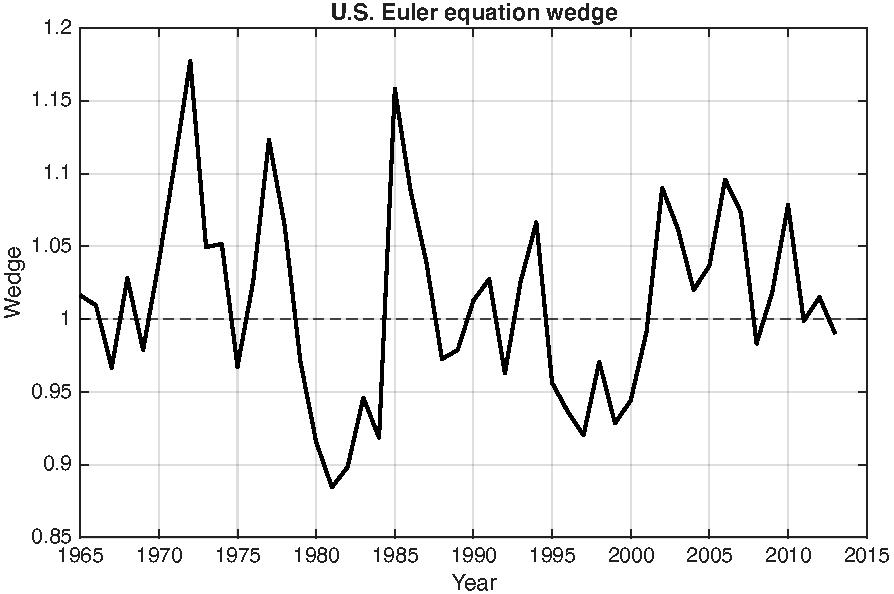
\includegraphics[width=0.72\textwidth]{../analysis/code/model/results/wedge.pdf}
\end{figure}

\end{document}
